\documentclass[aspectratio=169,11pt]{beamer}

\usefonttheme{professionalfonts}
\usepackage{fontspec}
\usepackage{unicode-math}

\def\FONTDIR{/Users/admin/Documents/thaitd/Code/giaoanMathtech/assets/fonts/}
\setmainfont{BeVietnamPro}[Path=\FONTDIR, Extension=.ttf,
  UprightFont=*-Regular, BoldFont=*-Bold, ItalicFont=*-Italic, FontFace={sb}{n}{*-SemiBold} ]
\setsansfont{BeVietnamPro}[Path=\FONTDIR, Extension=.ttf,
  UprightFont=*-Regular, BoldFont=*-Bold, ItalicFont=*-Italic ]
\setmathfont{STIXTwoMath-Regular.otf}[Path=\FONTDIR]

\usepackage{tikz}
\usetikzlibrary{calc,positioning,arrows.meta,shapes.geometric}
\usepackage{adjustbox}
\usepackage[most]{tcolorbox}
\usepackage{colortbl}
\usepackage{hyperref}

% Màu sắc nhận diện
\usepackage{xcolor}
\definecolor{brand}{HTML}{1E3A8A}      % Xanh Navy chủ đạo
\definecolor{accent}{HTML}{D97706}     % Vàng Cam nhấn
\definecolor{ink}{HTML}{1E293B}        % Chữ đậm
\definecolor{neutral}{HTML}{F8FAFC}    % Nền phụ
\definecolor{rule}{HTML}{E2E8F0}       % Kẻ ngang
\definecolor{muted}{HTML}{64748B}      % Chữ mờ
\definecolor{info}{HTML}{2563EB}       % Link xanh
\definecolor{success}{HTML}{15803D}    % Xanh lá
\definecolor{successbg}{HTML}{DCFCE7}  % Nền xanh lá
\definecolor{cardbg}{HTML}{F1F5F9}     % Nền card
\definecolor{danger}{HTML}{DC2626}     % Đỏ cảnh báo
\definecolor{dangerbg}{HTML}{FEE2E2}   % Nền đỏ
\definecolor{purple}{HTML}{7E22CE}     % Tím
\definecolor{purplebg}{HTML}{EDE7F6}   % Nền tím

\hypersetup{
  colorlinks=true,
  urlcolor=info,
  linkcolor=brand
}

\usetheme{default}
\setbeamertemplate{navigation symbols}{}
\setbeamercolor{normal text}{fg=ink}
\setbeamercolor{structure}{fg=brand}
\setbeamercolor{frametitle}{fg=brand}
\setbeamerfont{frametitle}{series=\bfseries, size=\large}
\setbeamerfont{normal text}{size=\small}

% Watermark
\newif\ifwatermark\watermarktrue
\setbeamertemplate{background}{%
  \ifwatermark
    \begin{tikzpicture}[remember picture,overlay]
      \node[opacity=0.15] at (current page.center)
        {\includegraphics[width=0.42\paperwidth]{/Users/admin/Documents/thaitd/Code/giaoanMathtech/assets/Watermark_Opacity_20.png}};
    \end{tikzpicture}%
  \fi}

% Header frametitle gọn gàng, tiết kiệm chiều cao
\setbeamertemplate{frametitle}{%
  \vspace*{4pt}\hspace*{0.1cm}{\usebeamerfont{frametitle}\usebeamercolor[fg]{frametitle}\insertframetitle}\par
  \vspace{1pt}\hspace*{0.1cm}{\color{accent}\rule{36pt}{1.8pt}}\par\vspace{1pt}}

% Footer
\setbeamertemplate{footline}{%
  \leavevmode%
  \hspace*{0.6cm}{\color{rule}\rule{\dimexpr\paperwidth-1.2cm\relax}{0.4pt}}\par\vspace{2pt}%
  \hbox to \paperwidth{%
    \hspace*{0.6cm}%
    \raisebox{-1pt}{\includegraphics[height=9pt]{/Users/admin/Documents/thaitd/Code/giaoanMathtech/assets/logo_mathtech_compact.png}}%
    \hspace*{6pt}{\scriptsize\color{muted}MathTech Engine • Thầy Trương Đình Thái}%
    \hfill%
    {\scriptsize\color{muted}Slide \insertframenumber{} / \inserttotalframenumber}%
    \hspace*{0.6cm}%
  }%
  \vskip3pt}

% Card styles - tối ưu đệm (padding) để không bao giờ tràn đáy
\tcbset{
  slidecard/.style={
    colback=neutral, colframe=rule, boxrule=0.7pt, arc=3pt,
    left=5pt, right=5pt, top=3pt, bottom=3pt,
    fonttitle=\bfseries\sffamily\footnotesize, coltitle=brand
  },
  accentcard/.style={
    colback=accent!6, colframe=accent, boxrule=0.7pt, arc=3pt,
    left=5pt, right=5pt, top=3pt, bottom=3pt,
    fonttitle=\bfseries\sffamily\footnotesize, coltitle=accent
  },
  successcard/.style={
    colback=successbg, colframe=success, boxrule=0.7pt, arc=3pt,
    left=5pt, right=5pt, top=3pt, bottom=3pt,
    fonttitle=\bfseries\sffamily\footnotesize, coltitle=success
  },
  dangercard/.style={
    colback=dangerbg, colframe=danger, boxrule=0.7pt, arc=3pt,
    left=5pt, right=5pt, top=3pt, bottom=3pt,
    fonttitle=\bfseries\sffamily\footnotesize, coltitle=danger
  },
  quotecard/.style={
    colback=white, colframe=brand!40, boxrule=0.6pt, arc=2pt,
    left=4pt, right=4pt, top=3pt, bottom=3pt
  }
}

\begin{document}

% ========================================================
% SLIDE 1: TIÊU ĐỀ
% ========================================================
\watermarkfalse
\begin{frame}[plain]
  \begin{tikzpicture}[remember picture,overlay]
    \fill[color=brand] (current page.north west) rectangle ([xshift=0.35in]current page.south west);
    \fill[color=accent] ([xshift=0.35in]current page.north west) rectangle ([xshift=0.38in]current page.south west);
  \end{tikzpicture}

  \vspace*{0.22in}
  \begin{flushleft}
    \hspace*{0.55in}
    \begin{minipage}{0.85\textwidth}
      \includegraphics[height=26pt]{/Users/admin/Documents/thaitd/Code/giaoanMathtech/assets/logo_mathtech_compact.png}\par\vspace{10pt}
      {\setlength{\fboxsep}{3pt}\colorbox{brand}{\color{white}\sffamily\bfseries\scriptsize\strut\,CẨM NANG NỘI BỘ DÀNH CHO GIÁO VIÊN MỚI\,}}\par\vspace{6pt}
      {\bfseries\LARGE\color{brand}HƯỚNG DẪN CÁCH SỬ DỤNG AI\\SOẠN PHIẾU HỌC TẬP \& HỆ THỐNG TEMPLATES}\par\vspace{6pt}
      {\color{accent}\rule{130pt}{2.5pt}}\par\vspace{6pt}
      {\color{muted}\small\sffamily Tư duy phân tầng sư phạm, Hệ thống 3 Template Sheets \& Quy trình 5 bước AI}\par
      \vspace{12pt}
      {\color{ink}\small\sffamily Người thuyết trình: \textbf{Trương Đình Thái} • Tổ Học Liệu MathTech}
    \end{minipage}
  \end{flushleft}
  \vfill
\end{frame}
\watermarktrue

% ========================================================
% SLIDE 2: TẢI TOOL, CÀI EXTENSION & MỞ CHAT AI
% ========================================================
\begin{frame}{Khởi Động Nhanh (3 Phút): Tải Tool, Extension \& Mở AI}
  \begin{columns}[T]
    \begin{column}{0.48\textwidth}
      \begin{tcolorbox}[slidecard, top=2pt, bottom=2pt, title=1. Tải Mã Nguồn \& Antigravity]
        \scriptsize
        • \textbf{Codebase MathTech (GitHub):}\\
        \href{https://github.com/icecubesssss/giaoanmathtech}{\textbf{\color{info}github.com/.../giaoanmathtech}}\\
        {\color{muted}(Bấm Code $\to$ Download ZIP $\to$ Giải nén)}\\[3pt]
        • \textbf{Ứng dụng AI Antigravity:}\\
        \href{https://antigravity.google/download}{\textbf{\color{info}antigravity.google/download}}
      \end{tcolorbox}
      \vspace{1pt}
      \begin{tcolorbox}[slidecard, top=2pt, bottom=2pt, title=2. Mở Thư Mục \& Kích Hoạt Môi Trường]
        \scriptsize
        Mở Antigravity $\to$ \textbf{Open Folder} trỏ vào code $\to$ Mở chat AI và nhắn:
        \vspace{1pt}
        \begin{center}
          \colorbox{white}{\color{accent}\bfseries\scriptsize "Cài đặt môi trường giúp tôi"}
        \end{center}
        {\color{success}\textbf{$\blacktriangleright$ AI tự cài Python \& thư viện từ A – Z!}}
      \end{tcolorbox}
    \end{column}

    \begin{column}{0.48\textwidth}
      \begin{tcolorbox}[accentcard, top=3pt, bottom=3pt, title=3. Cài 2 Extension Thiết Yếu (Trong VS Code)]
        \scriptsize
        Mở mục \textbf{Extensions} (\texttt{Ctrl+Shift+X} / \texttt{Cmd+Shift+X}):\\[2pt]
        \textbf{1. Extension Claude (Claude Code):}\\
        Dùng Claude tương tác trực tiếp, chạy lệnh soạn bài và phân dạng cùng AI.\\[4pt]
        \textbf{2. Extension vscode-pdf:}\\
        Mở và xem trực tiếp 3 bản PDF (Handout HS, Guide GV, Slide) ngay trong cửa sổ làm việc mà không cần cài thêm app ngoài.\\[4pt]
        {\color{brand}\textbf{Lợi ích:}} Toàn bộ thao tác chỉ diễn ra trong 1 màn hình duy nhất!
      \end{tcolorbox}
    \end{column}
  \end{columns}
\end{frame}

% ========================================================
% SLIDE 3: CƠ CHẾ HOẠT ĐỘNG
% ========================================================
\begin{frame}{Cơ Chế Hoạt Động: Inputs $\to$ Process $\to$ Outputs}
  \vspace{-3pt}
  \begin{center}
    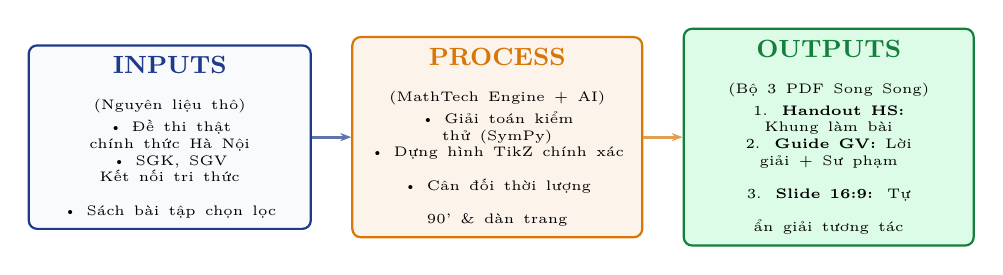
\begin{tikzpicture}[node distance=0.5cm, auto]
      \node[draw=brand, fill=neutral, rounded corners=3pt, line width=0.8pt, text width=3.3cm, align=center, inner sep=4pt] (in) {
        {\bfseries\color{brand}\small INPUTS}\\[1pt]
        {\tiny (Nguyên liệu thô)}\\[2pt]
        {\tiny • Đề thi thật chính thức Hà Nội\\• SGK, SGV Kết nối tri thức\\• Sách bài tập chọn lọc}
      };
      \node[draw=accent, fill=accent!8, rounded corners=3pt, line width=0.8pt, text width=3.4cm, align=center, inner sep=4pt, right=of in] (pro) {
        {\bfseries\color{accent}\small PROCESS}\\[1pt]
        {\tiny (MathTech Engine + AI)}\\[2pt]
        {\tiny • Giải toán kiểm thử (SymPy)\\• Dựng hình TikZ chính xác\\• Cân đối thời lượng 90' \& dàn trang}
      };
      \node[draw=success, fill=successbg, rounded corners=3pt, line width=0.8pt, text width=3.4cm, align=center, inner sep=4pt, right=of pro] (out) {
        {\bfseries\color{success}\small OUTPUTS}\\[1pt]
        {\tiny (Bộ 3 PDF Song Song)}\\[2pt]
        {\tiny 1. \textbf{Handout HS:} Khung làm bài\\2. \textbf{Guide GV:} Lời giải + Sư phạm\\3. \textbf{Slide 16:9:} Tự ẩn giải tương tác}
      };
      \draw[-{Stealth[length=4pt]}, line width=1pt, draw=brand!70] (in) -- (pro);
      \draw[-{Stealth[length=4pt]}, line width=1pt, draw=accent!70] (pro) -- (out);
    \end{tikzpicture}
  \end{center}
  \vspace{2pt}
  \begin{tcolorbox}[slidecard]
    \scriptsize\centering
    \textbf{[Mẹo]} \textbf{Giáo viên chỉ cần tập trung vào sư phạm} — AI tự động giải toán, vẽ hình và xuất trọn bộ PDF!
  \end{tcolorbox}
\end{frame}

% ========================================================
% SLIDE 4: PHÂN TẦNG NĂNG LỰC HỌC SINH
% ========================================================
\begin{frame}{Phân Tầng Năng Lực Học Sinh (A – B – C – X)}
  \begin{adjustbox}{max width=\textwidth}
    \begin{tabular}{|c|l|c|l|}
      \hline
      \rowcolor{brand!15}
      \textbf{Tầng} & \textbf{Đối tượng học sinh} & \textbf{Mục tiêu điểm} & \textbf{Giới hạn bài tập} \\
      \hline
      \rowcolor{brand!5}
      \textbf{\color{brand}C} & \textbf{Nền tảng trung bình – yếu}, hay quên & 7,0 – 8,0 điểm & \textbf{\color{danger}Trần: Vận dụng (CẤM VDC)} \\
      \hline
      \textbf{B} & Trung bình – khá, chắc cơ bản & 9,0 – 10 điểm & Có VDC nhẹ (ít hơn lớp A) \\
      \hline
      \textbf{A} & Khá – giỏi, tư duy tốt & Đạt điểm tối đa (10đ) & VDC dày dặn, mở rộng cấu hình \\
      \hline
      \textbf{\color{accent}X} & Chuyên Toán / Chất lượng cao & Chinh phục câu cuối đề & VDC nâng cao, cực trị, BĐT \\
      \hline
    \end{tabular}
  \end{adjustbox}
  \vspace{6pt}
  \begin{tcolorbox}[accentcard]
    \scriptsize
    \textbf{[Lưu ý]} \textbf{Trọng tâm hiện tại:} Toàn bộ phiếu học tập tập trung thiết kế cho \textbf{LỚP C} — nơi học sinh cần giàn giáo sư phạm vững chắc nhất để không bị bỏ lại phía sau!
  \end{tcolorbox}
\end{frame}

% ========================================================
% SLIDE 5: 4 CẤP ĐỘ CÂU HỎI
% ========================================================
\begin{frame}{4 Cấp Độ Câu Hỏi (NB – TH – VD – VDC)}
  \begin{columns}[T]
    \begin{column}{0.48\textwidth}
      \begin{tcolorbox}[slidecard, top=2pt, bottom=2pt, title=\textbf{NB (Nhận biết — 1 bước)}]
        \scriptsize
        Định nghĩa, công thức, tính nhẩm trực tiếp:\\
        • \textit{K3:} Tính nhẩm $7 \times 4 = 28$.\\
        • \textit{K6:} Tính giá trị $2^3 = 8$.\\
        • \textit{K9:} ĐKXĐ của $\sqrt{x-3}$; nhận diện góc vuông tiếp điểm.
      \end{tcolorbox}
      \vspace{1pt}
      \begin{tcolorbox}[successcard, top=2pt, bottom=2pt, title=\textbf{TH (Thông hiểu — 1–2 bước)}]
        \scriptsize
        Áp dụng quy tắc, định lý vào bài cơ bản:\\
        • \textit{K3:} "1 hộp 8 bánh, 3 hộp có bao nhiêu cái?"\\
        • \textit{K6:} Tính $A = 2^3 \cdot 5 - 3^2$.\\
        • \textit{K9:} Rút gọn biểu thức chứa căn; chứng minh $\triangle$ bằng nhau.
      \end{tcolorbox}
    \end{column}

    \begin{column}{0.48\textwidth}
      \begin{tcolorbox}[accentcard, top=2pt, bottom=2pt, title=\textbf{VD (Vận dụng — 2–3 bước)}]
        \scriptsize
        Bài toán thực tế, kết hợp nhiều phép tính:\\
        • \textit{K3:} "35 quả chia 5 túi, bán 2 túi, còn bao nhiêu?"\\
        • \textit{K6:} Tìm $x$ biết $2(x-3)^2 = 32$.\\
        • \textit{K9:} Chứng minh tiếp tuyến $DB \perp OB$; tính chiều cao TSLG.
      \end{tcolorbox}
      \vspace{1pt}
      \begin{tcolorbox}[dangercard, top=2pt, bottom=2pt, title=\textbf{VDC (Vận dụng cao — $\ge 4$ bước)}]
        \scriptsize
        Phân hóa điểm 9,5 – 10 (cực trị, hình phụ phức tạp):\\
        • Dành cho Lớp B, Lớp A và Lớp X.\\
        • \textbf{\color{danger}LỚP C: 0\% (TUYỆT ĐỐI CẤM ĐƯA VÀO PHIẾU!)}
      \end{tcolorbox}
    \end{column}
  \end{columns}
\end{frame}

% ========================================================
% SLIDE 6: KỸ THUẬT "NB TÁCH CÂU"
% ========================================================
\begin{frame}{Kỹ Thuật Then Chốt: "NB Tách Câu" (Giàn Giáo Lớp C)}
  \begin{tcolorbox}[dangercard]
    \scriptsize
    \textbf{\textbf{[CẢNH BÁO]} NGUYÊN TẮC VÀNG: CẤM DÙNG CÂU NB RỜI RẠC, VÔ BỔ!}\\
    Không ra các câu nhận diện hình thức kiểu "đây có phải là phương trình không?" hoặc tính toán máy móc không xuất hiện trong đề thi. Mọi câu NB bắt buộc phải là \textbf{bước đệm kỹ năng trích từ chính bài toán thi thật}.
  \end{tcolorbox}
  \vspace{2pt}
  \begin{columns}[T]
    \begin{column}{0.48\textwidth}
      \begin{tcolorbox}[slidecard, title=Bài Toán Đích Trong Đề Thi Thật]
        \scriptsize
        \textbf{Bài toán [TH]:} Tính giá trị biểu thức:
        \[ M = 150 - [100 - (3^2 \cdot 5)] \]
        {\color{muted}Học sinh lớp C thường lúng túng khi gặp ngoặc lồng ngoặc và lũy thừa $\to$ dễ bỏ cuộc.}
      \end{tcolorbox}
    \end{column}

    \begin{column}{0.48\textwidth}
      \begin{tcolorbox}[successcard, title=Chẻ Giàn Giáo Leo Dốc (Scaffolding)]
        \scriptsize
        • \textbf{Ý a [NB đệm]:} Tính giá trị của $3^2$ và $3^2 \cdot 5$.\\[3pt]
        • \textbf{Ý b [TH]:} Tính ngoặc vuông $[100 - (3^2 \cdot 5)]$ rồi tính $M$.\\[5pt]
        {\color{success}\textbf{$\blacktriangleright$ Hiệu quả:}} HS làm được ngay ý a, tự tin giải quyết trọn vẹn cả bài!
      \end{tcolorbox}
    \end{column}
  \end{columns}
\end{frame}

% ========================================================
% SLIDE 7: TỈ LỆ CHUẨN LỚP C
% ========================================================
\begin{frame}{Tỉ Lệ Chuẩn Lớp C: 40\% NB – 40\% TH – 20\% VD}
  \begin{columns}[T]
    \begin{column}{0.48\textwidth}
      \begin{tcolorbox}[slidecard, title=Công Thức Phân Bổ Năng Lực]
        \scriptsize
        • \textbf{40\% Nhận biết (NB):} Xây chắc kỹ năng cơ bản, tạo đà tâm lý.\\[3pt]
        • \textbf{40\% Thông hiểu (TH):} Áp dụng công thức, rèn tính cẩn thận.\\[3pt]
        • \textbf{20\% Vận dụng (VD):} Va chạm bài toán thực tế vừa sức.\\[3pt]
        • \textbf{0\% Vận dụng cao (VDC):} Tránh gây quá tải và sợ hãi.
      \end{tcolorbox}
    \end{column}

    \begin{column}{0.48\textwidth}
      \begin{tcolorbox}[accentcard, title=Định Mức Thời Lượng Ca Học 90 Phút]
        \scriptsize
        • \textbf{GV Giảng \& Ví dụ mẫu:} 25 phút.\\[3pt]
        • \textbf{HS Luyện tập trên lớp:} 55 phút (nghỉ giải lao 10').\\[3pt]
        • \textbf{BTVN tự luyện tại nhà:} 40 phút.\\[3pt]
        {\color{muted}(Định mức K9: 1,5'/câu NB • 6'/câu TH • 12'/câu VD • Vẽ hình +5').}
      \end{tcolorbox}
    \end{column}
  \end{columns}
  \vspace{3pt}
  \begin{tcolorbox}[slidecard]
    \centering\scriptsize
    \textbf{TỈ LỆ THỜI GIAN LỚP C (120'):} {\color{brand}\textbf{48' NB (40\%)}} • {\color{success}\textbf{48' TH (40\%)}} • {\color{accent}\textbf{24' VD (20\%)}} • {\color{danger}\textbf{0' VDC (0\%)}}
  \end{tcolorbox}
\end{frame}

% ========================================================
% SLIDE 8: CẤU TRÚC 4 CHẶNG TRÊN PHIẾU
% ========================================================
\begin{frame}{Cấu Trúc 4 Chặng Sư Phạm Của 1 Phiếu Học Tập}
  \begin{adjustbox}{max width=\textwidth}
    
\begin{tikzpicture}[node distance=0.25cm, auto]
      \tikzset{
        stage/.style={draw=brand, fill=neutral, rounded corners=3pt, line width=0.7pt, text width=2.9cm, align=center, inner sep=4pt, font=\sffamily\scriptsize},
        stagearrow/.style={-{Stealth[length=4pt]}, line width=1pt, draw=brand!70}
      }
      \node[stage] (c1) {{\bfseries\color{brand}CHẶNG 1: NỀN}\\[1pt]{\tiny Ôn kỹ năng lớp dưới/bài trước}};
      \node[stage, right=of c1] (c2) {{\bfseries\color{brand}CHẶNG 2: MỚI}\\[1pt]{\tiny Công thức, quy tắc ngắn gọn}};
      \node[stage, right=of c2] (c3) {{\bfseries\color{brand}CHẶNG 3: MẪU}\\[1pt]{\tiny GV làm mẫu (điền khuyết)}};
      \node[stage, right=of c3] (c4) {{\bfseries\color{brand}CHẶNG 4: LUYỆN}\\[1pt]{\tiny HS tự làm (LT1 $\to$ LT2)}};

      \draw[stagearrow] (c1) -- (c2);
      \draw[stagearrow] (c2) -- (c3);
      \draw[stagearrow] (c3) -- (c4);
    \end{tikzpicture}
  \end{adjustbox}
  \vspace{8pt}
  \begin{tcolorbox}[slidecard]
    \scriptsize
    \textbf{[Ghi chú]} \textbf{Tư duy dạy học:} Thầy cô lên lớp chỉ cần giảng đúng theo thứ tự 4 chặng này — tài liệu đã được dàn trang và lập trình sẵn để học sinh tiếp thu tự nhiên nhất.
  \end{tcolorbox}
\end{frame}

% ========================================================
% SLIDE 9: QUY TRÌNH 5 BƯỚC SOẠN PHIẾU CÙNG AI
% ========================================================
\begin{frame}{Quy Trình 5 Bước Soạn Phiếu Cùng AI}
  \vspace{-3pt}
  \begin{center}
    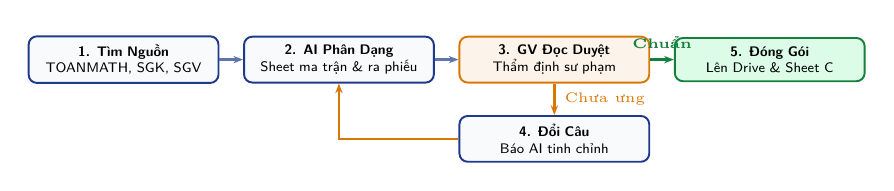
\begin{tikzpicture}[node distance=0.3cm, auto]
      \tikzset{
        wfstep/.style={draw=brand, fill=neutral, rounded corners=3pt, line width=0.7pt, text width=2.2cm, align=center, inner sep=3pt, font=\sffamily\tiny},
        wfarrow/.style={-{Stealth[length=3.5pt]}, line width=0.9pt, draw=brand!70}
      }
      \node[wfstep] (s1) {\textbf{1. Tìm Nguồn}\\TOANMATH, SGK, SGV};
      \node[wfstep, right=of s1] (s2) {\textbf{2. AI Phân Dạng}\\Sheet ma trận \& ra phiếu};
      \node[wfstep, draw=accent, fill=accent!8, right=of s2] (s3) {\textbf{3. GV Đọc Duyệt}\\Thẩm định sư phạm};
      \node[wfstep, draw=success, fill=successbg, right=of s3] (s5) {\textbf{5. Đóng Gói}\\Lên Drive \& Sheet C};
      \node[wfstep, below=0.4cm of s3] (s4) {\textbf{4. Đổi Câu}\\Báo AI tinh chỉnh};

      \draw[wfarrow] (s1) -- (s2);
      \draw[wfarrow] (s2) -- (s3);
      \draw[wfarrow, draw=success] (s3) -- node[above, font=\tiny\bfseries\color{success}] {Chuẩn} (s5);
      \draw[wfarrow, draw=accent] (s3) -- node[right, font=\tiny\color{accent}] {Chưa ưng} (s4);
      \draw[wfarrow, draw=accent] (s4) -| (s2);
    \end{tikzpicture}
  \end{center}
  \vspace{1pt}
  \begin{tcolorbox}[slidecard]
    \scriptsize
    \textbf{Tách bạch vai trò:} Con người kiểm soát mục tiêu sư phạm \& chất lượng đề $\longleftrightarrow$ AI phụ trách quét dữ liệu, tính toán định mức và biên dịch tài liệu.
  \end{tcolorbox}
\end{frame}

% ========================================================
% SLIDE 10: HỆ THỐNG 3 TEMPLATE SHEETS LIÊN KẾT ĐỘNG
% ========================================================
\begin{frame}{Hệ Thống 3 Template Sheets Liên Kết Động Trong MathTech}
  \vspace{-5pt}
  \begin{center}
    \scriptsize\colorbox{brand!10}{%
      \textbf{$\blacktriangleright$ Link Google Sheets Mẫu Chuẩn:}
      \href{https://docs.google.com/spreadsheets/d/1ARD_4AKM_aXlyGz3tOCoUYjOEnlOgXCmcO0ISeK6boY/edit}{\textbf{\color{info}Bấm vào đây để mở Spreadsheet mẫu (Tạo bản sao)}}%
    }
  \end{center}
  \vspace{1pt}
  \begin{columns}[T]
    \begin{column}{0.485\textwidth}
      \begin{tcolorbox}[slidecard, top=2pt, bottom=2pt, title=Template 1 \& 2: Thiết Kế \& Phân Dạng]
        \scriptsize
        • \textbf{Template 1 (Tab Phân Dạng 47 Cột):}\\
        Ngân hàng đề quét sạch, tự động lọc L1–L5 và chấm điểm T1–T8.\\[2pt]
        • \textbf{Template 2 (Tab Thuyết Minh Động):}\\
        Bản spec buổi học, cân đối 40-40-20 và quỹ thời lượng 90'.
      \end{tcolorbox}
    \end{column}

    \begin{column}{0.485\textwidth}
      \begin{tcolorbox}[successcard, top=2pt, bottom=2pt, title=Template 3: Bàn Giao \& Tiến Độ]
        \scriptsize
        • \textbf{Template 3 (Sheet Tiến Độ):}\\
        Quản lý tiến độ tuần, đồng bộ trọn bộ link Drive (Handout, Guide, Slide).\\[2pt]
        • \textbf{Quy chuẩn Đề thi:}\\
        {\color{muted}Đề thi do Thầy tạo riêng. GV và AI hoàn thiện 3 template bài giảng.}
      \end{tcolorbox}
    \end{column}
  \end{columns}
  \vspace{1pt}
  \begin{tcolorbox}[accentcard, top=2pt, bottom=2pt]
    \centering\scriptsize
    \textbf{Nguyên tắc cốt lõi:}\par\vspace{1pt}
    [T1: Ngân hàng 47 cột] $\xrightarrow{\text{Mã câu}}$ [T2: Spec] $\xrightarrow{\text{Duyệt}}$ [Bộ 3 PDF] $\xrightarrow{\text{Đóng gói}}$ [T3: Tiến độ Drive]
  \end{tcolorbox}
\end{frame}

% ========================================================
% SLIDE 11: TEMPLATE 1 - TAB PHÂN DẠNG 47 CỘT
% ========================================================
\begin{frame}{Template 1: Tab Phân Dạng Chương (47 Cột Chuẩn)}
  \vspace{-3pt}
  \begin{columns}[T]
    \begin{column}{0.485\textwidth}
      \begin{tcolorbox}[slidecard, top=3pt, bottom=3pt, title={Phân Khu I, II, III: Thiết Kế \& Giàn Giáo}]
        \scriptsize
        • \textbf{\color{brand}I. Dữ liệu đề thô (Cột A -- M):}\\
        Chép nguyên văn từ đề thật; gồm `Bài cụ thể`, `Nguồn`, `Mức độ`, `Dạng bài`, `Thời lượng`, \textbf{`Mã câu` (M)} (khóa định danh duy nhất).\\[3pt]
        • \textbf{\color{accent}II. Giàn giáo §4b (Cột N -- X):}\\
        Gán 7 loại câu §4b (`NB lẻ LT`, `NB tách TH`, `TH tách VD`...); tự động xếp C/B/X; bộ lọc \textbf{`Loại ngay (L1--L5)`}; vùng \textit{`Chọn tay`}.\\[3pt]
        • \textbf{III. Bóc tách ý con (Cột Y -- AE):}\\
        Tách bài VD thành chuỗi bước đệm TH $\to$ NB; `Mã bài gốc`, `Kỹ thuật giải`, `Chương ([V])`, `Nhóm trùng`.
      \end{tcolorbox}
    \end{column}

    \begin{column}{0.485\textwidth}
      \begin{tcolorbox}[successcard, top=3pt, bottom=3pt, title={Phân Khu IV, V: Đánh Giá \& Kết Luận}]
        \scriptsize
        • \textbf{\color{success}IV. Chấm 8 tiêu chí chất lượng (AF -- AM):}\\
        Chấm 0, 1, 2 cho T1 Trọng tâm SGK $\dots$ T8 Mở rộng: Đánh giá ý toán trong sáng, nghiệm đẹp, bẫy lỗi sai kinh điển.\\[3pt]
        • \textbf{\color{danger}V. Đánh giá phân tầng (AN -- AU):}\\
        Tính điểm C/B/X, so ngưỡng mức AQ $\to$ Kết luận: \textit{Đưa vào bài / Dự phòng / Loại}. \textbf{THẦY DUYỆT} chốt chặn.\\[4pt]
        \tcblower
        \tiny
        \textbf{[Mẹo]} \textbf{Mã màu:} {\color{accent}Cam: VD/VDC} • {\color{brand}Vàng: Thầy chọn} • {\color{success}Xanh: Vào bài} • {\color{purple}Tím: NB cũ} • {\color{danger}Đỏ: Loại}.
      \end{tcolorbox}
    \end{column}
  \end{columns}
\end{frame}

% ========================================================
% SLIDE 12: CƠ CHẾ LỌC L1-L5 VÀ CHẤM T1-T8
% ========================================================
\begin{frame}{Cơ Chế Lọc Loại Ngay (L1–L5) \& Chấm Điểm (T1–T8)}
  \begin{columns}[T]
    \begin{column}{0.48\textwidth}
      \begin{tcolorbox}[dangercard, title=Bộ Lọc Loại Ngay L1–L5 (Cột Q)]
        \scriptsize
        • \textbf{L1:} Sai kiến thức toán / giả thiết ngớ ngẩn.\\[2pt]
        • \textbf{L2:} Lệch chuẩn chương trình SGK GDPT 2018.\\[2pt]
        • \textbf{L3:} Nghiệm cồng kềnh, số lẻ vô tỉ xấu.\\[2pt]
        • \textbf{L4:} Quá 4 bước suy luận không thể tách giàn giáo.\\[2pt]
        • \textbf{L5:} Trùng ý chỉ đổi số trên lớp (chỉ cho phép ở BTVN).
      \end{tcolorbox}
    \end{column}

    \begin{column}{0.48\textwidth}
      \begin{tcolorbox}[successcard, title=Công Thức Chấm Điểm Lớp C (Cột AN \& AR)]
        \scriptsize
        \vspace{-2pt}
        {\footnotesize \[ \text{Điểm}_C = \frac{\sum (T_i \times W_i)}{2 \times 13} \times 10 \]}
        \vspace{-4pt}
        {\tiny ($W_C$: $3T_1 + 1T_2 + 2T_3 + 1T_4 + 2T_5 + 2T_6 + 2T_7 + 0T_8$)}\\[2pt]
        • \textbf{Ngưỡng đưa vào bài (AQ):}\\
        $\text{VD} \ge 7{,}0$ • $\text{TH} \ge 6{,}0$ • $\text{NB} \ge 5{,}0$.\\[2pt]
        • \textbf{Công thức tự động (AR):}\\
        {\scriptsize\texttt{=IF(Q6<>"","LOẠI",IF(V6<>"","CHỌN TAY",...))}}\\[1pt]
        {\tiny Tự động: \textit{Đưa vào bài / Dự phòng / Loại}.}
      \end{tcolorbox}
    \end{column}
  \end{columns}
\end{frame}

% ========================================================
% SLIDE 13: TEMPLATE 2 - THUYẾT MINH SPEC ĐỘNG
% ========================================================
\begin{frame}{Template 2: Tab Thuyết Minh Liên Kết Động (Spec Sheet)}
  \begin{columns}[T]
    \begin{column}{0.48\textwidth}
      \begin{tcolorbox}[slidecard, title=Cấu Trúc Ma Trận Dạng Bài]
        \scriptsize
        • \textbf{Loại câu (§4b):} 7 nhãn chuẩn (NB lẻ LT, NB tách TH, TH ghép VD, VD lẻ...) + NB kiến thức cũ.\\[3pt]
        • \textbf{Dạng bài:} Tên dạng toán chuẩn (bọc $\$...\$$).\\[3pt]
        • \textbf{Mã câu đề xuất:} Trỏ trực tiếp cột Mã câu (M) của Template 1.\\[3pt]
        • \textbf{THẦY CHỌN \& ĐỔI CÂU:} Vùng Thầy nhập mã câu mới.\\[3pt]
        • \textbf{Chốt mã:} \texttt{=IF(Thầy\_Chọn<>"", Thầy\_Chọn, Đề\_Xuất)}
      \end{tcolorbox}
    \end{column}

    \begin{column}{0.48\textwidth}
      \begin{tcolorbox}[accentcard, title=Gác Cổng Tự Động (thuyetminh\_gate)]
        \scriptsize
        • Tự động chặn nếu quỹ giờ lệch quá $\pm 10\%$.\\[3pt]
        • Tự động chặn nếu xuất hiện câu VDC ở Lớp C.\\[3pt]
        • Cảnh báo nếu thiếu khai báo nhãn Loại câu §4b.\\[3pt]
        • Tự động kiểm tra liên kết mã câu với Tab Phân dạng.\\[4pt]
        {\color{success}\textbf{Định mức ca 90':}} GV giảng 25' • HS luyện 55' • BTVN 40'.
      \end{tcolorbox}
    \end{column}
  \end{columns}
\end{frame}

% ========================================================
% SLIDE 14: TEMPLATE 3 - SHEET TIẾN ĐỘ & DRIVE
% ========================================================
\begin{frame}{Template 3: Sheet Quản Trị Tiến Độ \& Đồng Bộ Drive}
  \begin{columns}[T]
    \begin{column}{0.48\textwidth}
      \begin{tcolorbox}[slidecard, title=Cấu Trúc Quản Trị Tiến Độ Tuần]
        \scriptsize
        • \textbf{Thông tin ca học:} Tuần/Ca $\to$ Mã phiếu $\to$ Tên bài SGK.\\[3pt]
        • \textbf{Hồ sơ gốc:} Link Sheet Phân dạng $\to$ Link Thuyết minh PDF.\\[3pt]
        • \textbf{Trạng thái duyệt:} [Soạn] Đang soạn $\to$ [Chờ duyệt] Chờ duyệt $\to$ [ĐÃ DUYỆT] \textbf{ĐÃ DUYỆT}.\\[3pt]
        • \textbf{Nghiệm thu:} Tích xanh checkbox khi bàn giao in ấn cho cơ sở.
      \end{tcolorbox}
    \end{column}

    \begin{column}{0.48\textwidth}
      \begin{tcolorbox}[successcard, title=Đồng Bộ 100\% Lên Google Drive]
        \scriptsize
        • \textbf{Link Handout HS:} Bản in có sẵn khung làm bài.\\[3pt]
        • \textbf{Link Guide GV:} Bản có đáp án + gợi ý sư phạm.\\[3pt]
        • \textbf{Link Slide Beamer:} File trình chiếu tương tác 16:9.\\[3pt]
        • \textbf{Link File Nguồn:} Mã nguồn phiếu JSON + TeX lưu trữ.
      \end{tcolorbox}
    \end{column}
  \end{columns}
  \vspace{2pt}
  \begin{tcolorbox}[accentcard]
    \centering\scriptsize
    \textbf{[Ghi chú]} Khi GV duyệt xong, chỉ cần nhắn AI: \textit{"Hãy đưa lên Drive và cập nhật Sheet Tiến độ giúp tôi"} $\to$ AI tự làm 100\%!
  \end{tcolorbox}
\end{frame}

% ========================================================
% SLIDE 15: THỰC HÀNH BƯỚC 1 & 2
% ========================================================
\begin{frame}{Thực Hành Bước 1 \& 2: Tìm Nguồn \& AI Phân Dạng}
  \begin{columns}[T]
    \begin{column}{0.48\textwidth}
      \begin{tcolorbox}[slidecard, title=BƯỚC 1: Chuẩn Bị Inputs Nguồn]
        \scriptsize
        • Đề thi chính thức các trường Hà Nội:\\
        \href{https://thcs.toanmath.com}{\textbf{\color{info}thcs.toanmath.com}}\\[4pt]
        • Ảnh scan SGK, SGV Kết nối tri thức (có sẵn trong kho).\\[4pt]
        • Sách bài tập \& đề thi học kỳ chuẩn hóa các năm gần nhất.
      \end{tcolorbox}
    \end{column}

    \begin{column}{0.48\textwidth}
      \begin{tcolorbox}[accentcard, title=BƯỚC 2: AI Quét Đề \& Lập Template 1 \& 2]
        \scriptsize
        Đưa đề cho AI đọc và quét trực tiếp vào Google Sheets:
        \vspace{2pt}
        \begin{tcolorbox}[quotecard]
          \color{brand}\itshape\tiny
          "Hãy quét các file đề thi HK1 trong thư mục inputs và điền vào Template 1 phân dạng Chương 5 giúp tôi. Chấm điểm T1-T8 cho lớp C."
        \end{tcolorbox}
        \vspace{1pt}
        {\color{success}\textbf{$\blacktriangleright$ AI tự làm:}} Chấm mã câu, gán nhãn §4b, chấm T1–T8, tính kết luận Lớp C và tạo dự thảo Template 2 (Thuyết minh).
      \end{tcolorbox}
    \end{column}
  \end{columns}
\end{frame}

% ========================================================
% SLIDE 16: THỰC HÀNH BƯỚC 3 & 4
% ========================================================
\begin{frame}{Thực Hành Bước 3 \& 4: Thẩm Định Sư Phạm \& Đổi Câu}
  \begin{columns}[T]
    \begin{column}{0.48\textwidth}
      \begin{tcolorbox}[accentcard, title=BƯỚC 3: GV Thẩm Định Sư Phạm]
        \scriptsize
        Mở bản in PDF Thuyết minh và đối chiếu 2 câu hỏi lớn:\\[3pt]
        1. \textit{"Trên lớp thực tế 90', mình có dẫn dắt HS lớp C học kịp phiếu này không?"}\\[4pt]
        2. \textit{"Các câu NB đệm có dẫn dắt mượt mà đến câu VD đích không?"}
      \end{tcolorbox}
    \end{column}

    \begin{column}{0.48\textwidth}
      \begin{tcolorbox}[slidecard, title=BƯỚC 4: Đổi Câu Linh Hoạt]
        \scriptsize
        Nếu câu quá khó hoặc bài khô khan, có 2 cách đổi:\\
        • \textbf{Cách 1:} Gõ mã câu mới vào cột \textit{THẦY CHỌN} ở Template 2.\\
        • \textbf{Cách 2:} Nhắn trực tiếp trong ô chat AI:
        \vspace{2pt}
        \begin{tcolorbox}[quotecard]
          \color{brand}\itshape\tiny
          "Câu 3 phần Luyện tập hơi khó so với lớp C, hãy chọn câu khác cùng dạng từ ngân hàng đề giúp tôi."
        \end{tcolorbox}
      \end{tcolorbox}
    \end{column}
  \end{columns}
\end{frame}

% ========================================================
% SLIDE 17: THỰC HÀNH BƯỚC 5
% ========================================================
\begin{frame}{Thực Hành Bước 5: Đóng Gói, Lên Drive \& Cập Nhật Tiến Độ}
  \begin{tcolorbox}[successcard]
    \scriptsize\centering
    \textbf{KHI PHIẾU ĐÃ CHUẨN 100\% — GV CHỈ CẦN RA LỆNH MỘT CHẠM CHO AI:}\\
    \colorbox{white}{\parbox{0.92\linewidth}{\centering\color{success}\bfseries\scriptsize "Phiếu 2 Chương 5 đã duyệt xong, hãy đưa lên Drive và cập nhật Template 3 (Sheet Tiến độ) giúp tôi."}}
  \end{tcolorbox}
  \vspace{1pt}
  \begin{columns}[T]
    \begin{column}{0.48\textwidth}
      \begin{tcolorbox}[slidecard, title=1. Tự Động Build \& Xuất Bản]
        \scriptsize
        AI tự chạy gác cổng nghiệm (SymPy) $\to$ render song song 3 bản PDF (Handout HS, Guide GV, Slide Beamer) $\to$ tải lên đúng thư mục Google Drive.
      \end{tcolorbox}
    \end{column}

    \begin{column}{0.48\textwidth}
      \begin{tcolorbox}[slidecard, title=2. Cập Nhật Sheet Tiến Độ]
        \scriptsize
        AI tự động điền URL Google Drive vào các cột Handout, Guide, Slide và tích xanh nghiệm thu hoàn thành.
      \end{tcolorbox}
    \end{column}
  \end{columns}
\end{frame}

% ========================================================
% SLIDE 18: TỔNG KẾT & CHEAT-SHEET
% ========================================================
\begin{frame}{Tổng Kết: Hệ Sinh Thái Sản Phẩm \& Cheat-Sheet Lệnh AI}
  \begin{columns}[T]
    \begin{column}{0.48\textwidth}
      \begin{tcolorbox}[slidecard, title=Hệ Sinh Thái Hoàn Thành Mỗi Chương]
        \scriptsize
        • \textbf{Template 1:} Ngân hàng đề 47 cột chấm điểm T1–T8.\\
        • \textbf{Template 2:} Phiếu Thuyết minh cân đối 40-40-20.\\
        • \textbf{Bộ 3 PDF Song Song:} Handout HS + Guide GV + Slide.\\
        • \textbf{Template 3:} Sheet Tiến độ tích xanh đồng bộ Drive.
      \end{tcolorbox}
    \end{column}

    \begin{column}{0.48\textwidth}
      \begin{tcolorbox}[accentcard, title=Cheat-Sheet Câu Lệnh Cho Giáo Viên]
        \scriptsize
        • \texttt{make b}: Build 3 PDF cho phiếu vừa làm (~9s).\\
        • \texttt{make check-tm}: Gác cổng thời lượng \& số câu.\\
        • \textit{"Cài đặt môi trường giúp tôi"}: Cài đặt tự động.\\
        • \textit{"Đổi câu X sang câu Y"}: Đổi câu tức thì.\\
        • \textit{"Đưa lên Drive và cập nhật Sheet"}: Hoàn tất buổi học.
      \end{tcolorbox}
    \end{column}
  \end{columns}
  \vspace{2pt}
  \begin{tcolorbox}[slidecard]
    \centering\tiny\color{muted}
    MathTech Engine 2026 — Đồng hành cùng Thầy Cô kiến tạo học liệu chuẩn mực, truyền cảm hứng cho mọi học sinh!
  \end{tcolorbox}
\end{frame}

\end{document}
